\documentclass[12pt]{article}
\usepackage{xcolor}
\usepackage{graphicx}
\usepackage{appendix}
\usepackage{verbatim}
\usepackage[margin=1.0in]{geometry}
\DeclareGraphicsExtensions{.jpg,.jpeg,.png}
\renewcommand{\baselinestretch}{1.0}
\begin{document}
\title{Simple Model of Cell Growth on a Stationary Nutrient Medium}
\author{Written by a cast of thousands}
\maketitle

% Change table counter
\renewcommand{\thetable}{\Roman{table}}

\section{Model}
This document describes the initial model implemented with the BoltzmannMFX
framework. This model is an extremely simplified model of microbial growth
designed to illustrated how the different components of the BoltzmannMFX
framework fit together and interact with each other. The cells consist of simple
circular disks that form a single layer on top of a stationary growth medium
(e.g. agar) and are fed by a single component ``nutrient''. The cells absorb the
nutrient and grow. When they reach a certain size, they split into two new
cells.

\begin{figure}
\centering
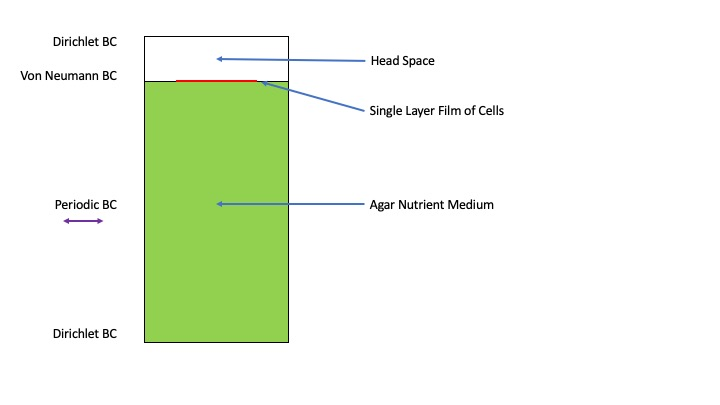
\includegraphics[width=4.0in,keepaspectratio=true]{FullSys}
\caption{\label{fullsys} Schematic diagram of the model growth region.}
\end{figure}
The geometry of the system is illustrated in figure (\ref{fullsys}) and shows a
rectangular volume that is square in cross section and elongated along one axis.
the system is periodic along the short axes. The long axis is divided into two
regions, one consisting of the stationary growth region and the other consisting
of a non-participating ``head-space''. The nutrient concentration is maintained
at a fixed value at the bottom of the system, corresponding to a Dirichlet
boundary condition. The top of the growth medium is impermeable to the nutrient,
so it should be characterized by a Von Neumann boundary condition representing
a zero normal gradient for the nutrient concentration. The head space does not
contain any chemical species and for this problem does not participate in any
significant way. The cells grow on top of the nutrient support layer in a
two-dimensional pattern.

\begin{figure}
\centering
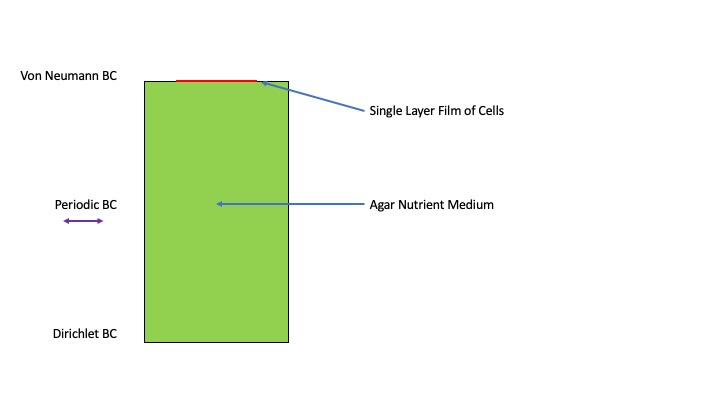
\includegraphics[width=4.0in,keepaspectratio=true]{ReducedSys}
\caption{\label{reducedsys} Schematic diagram of the model growth region with
head space removed.}
\end{figure}
Because the head space does not participate in any substantial way in this
model, it is possible to eliminate it entirely and use the geometry shown in
figure (\ref{reducedsys}). This eliminates an internal boundary and should make
development easier, but may gloss over an issue that will need to be dealt with
later as the model becomes more realistic.

\end{document}
